\section{Localização dos Usuários}
\label{sec:testes-localizacao}

O Sistema TRUE obtém a localização dos usuários no ambiente por meio de
coordenadas dos mesmos em relação ao \textit{Kinect}. Para verificar a acurácia
dessas coordenadas foram realizados alguns testes. Os resultados desses testes
foram desmostrados graficamente afim de comparar os dados obtidos
pelo sistema com os dados reais.

As coordenadas $\displaystyle (x, y, z)$ obtidas pelo sistema são coordenadas de
um plano cartesiano de três dimensões em que o ponto $\displaystyle (0, 0, 0)$
corresponde a posição do \textit{Kinect}. A coordenada no eixo  $\displaystyle
z$ mostra o quanto o usuário está distante, em termos de profundidade, em
relação ao sensor, a coordenada no eixo  $\displaystyle x$ mostra o quanto o
usuário está a direita ou a esquerda do sensor e a coordenada no eixo 
$\displaystyle y$ mostra o quanto o centro de massa geométrico do usuário está
acima ou abaixo do sensor.

Durante a estimativa da localização do usuário no ambiente inteligente, as
coordenadas no eixo  $\displaystyle y$ são ignoradas por que em contextos
ubíquos a localização espacial é baseada em ambientes (sala de
reunião 101, casa, patio, por exemplo) e não em relação a pontos cartesianos
gerais. Portanto, os testes desenvolvidos aferiram somente os valores obtidos
pelo Sistema TRUE nos eixos $\displaystyle x$ e $\displaystyle z$.

% Os valores das coordenadas que realmente são utilizadas para estimar a localização do usuário no ambiente são os valores nos eixos $\displaystyle x$ e $\displaystyle z$. Os valores do eixo $\displaystyle y$ correspondem somente a altura do centro de massa geométrico do usuário rastreado. 
\subsection{Teste de localização para o eixo $\displaystyle z$}

	Os valores obtidos no eixo $\displaystyle z$ correspondem aos valores de
	profundidade do usuário rastreado em relação ao \textit{Kinect}. Portanto, para
	testar a precisão do Sistema TRUE foi realizado o seguinte teste: um objeto (uma
	caixa de papelão) foi colocada em frente ao sensor a diferentes distâncias do
	mesmo (1000mm, 2000mm, 3000mm, 4000mm, 4057mm), como mostrado
	na Figura~\ref{fig:distancias}. Para distâncias acima de 4057mm não foram
	obtidos resultados, mais adiante, nessa seção, será provado que essa é a
	distância máxima de funcionamento do sensor. Para cada distância, foram
	coletados os dados informados pelo sistema. A Tabela~\ref{tab:valores-z}
	apresenta o comparativo entre as distâncias reais medidas manualmente e a
	média das distâncias aferidas pelo sistema. Essa média aritmética é calculada
	a partir das amostras coletadas em um determinado período de tempo sendo
	algumas dessas escolhidas aleatoriamente para fazer parte da operação.

	% \begin{figure}[htb]
	% 	\begin{center}
	% 		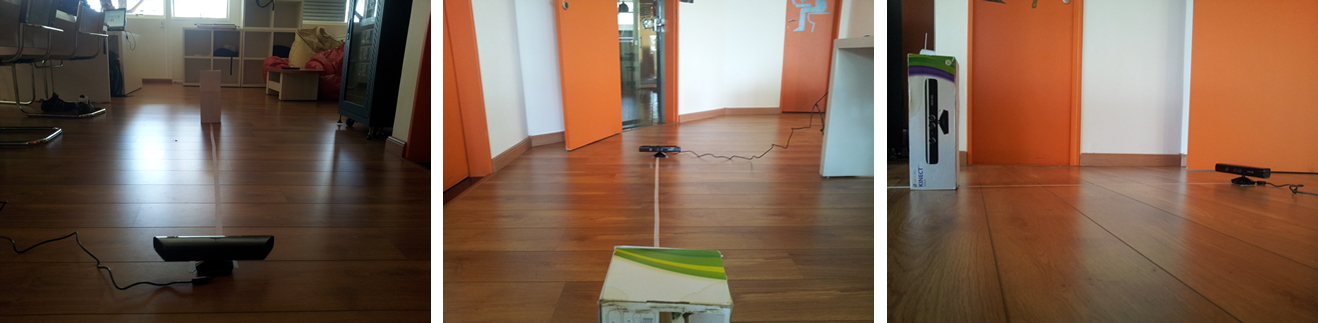
\includegraphics[scale=0.35]{figuras/5.Testes/teste-eixoz.png}
	% 	\end{center}
	% 	\caption{Fotos retiradas no teste realizado para aferir os valores obtidos no eixo $\displaystyle z$.}
	% 	\label{fig:teste-z}
	% \end{figure}

	\begin{figure}[htb]
		\begin{center}
			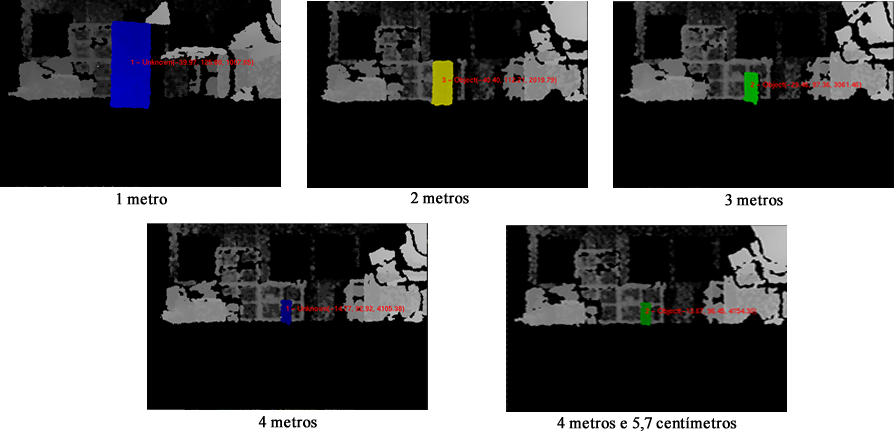
\includegraphics[width=0.95\textwidth]{figuras/5.Testes/eixoz-imgs2.png}
		\end{center}
		\caption{Fotos obtidas pelo Sistema TRUE nos testes de localização para o eixo $\displaystyle z$.}
		\label{fig:distancias}
	\end{figure}

	\begin{table}[h]
		\begin{center}
			\caption{Comparativo entre os valores reais e os valores obtidos pelo Sistema
			TRUE para o eixo $\displaystyle z$.}
			\label{tab:valores-z}
			\begin{tabular}{|c|c|}
				\hline \bf Distância real do objeto & \bf Média dos valores obtidos\\
							 \bf ao \textit{Kinect} (mm) & \bf pelo Sistema TRUE (mm)\\

				\hline
				\hline 1000,00 & 1006,24 \\ %1007,56 & 1006,64 & 1003,21 & 1007,56 \\
				\hline 2000,00 & 2020,62 \\ % 2020,27 & 2021,17 & 2020,55 & 2020,48 \\
				\hline 3000,00 & 3059,35 \\ % 3058,70 & 3057,60 & 3062,01 & 3059,10 \\
				\hline 4000,00 & 4112,99 \\ %4115,31 & 4110,25 & 4111,59 & 4114,80 \\
				\hline 4057,00 & 4166,34 \\ %4166,35 & 4163,83 & 4166,45 & 4168,75 \\
				\hline
			\end{tabular}
		\end{center}
	\end{table}

	Os valores da Tabela~\ref{tab:valores-z} também estão demostrados graficamente
	pela Figura~\ref{fig:grafico-z}. Como pode ser observado, a discrepância
	aumenta conforme o objeto se distancia do sensor. Neste teste o menor erro
	obtido foi de 3,21mm e o maior de 111,75mm.
	
	Pelos resultados dos testes de localização, pode-se concluir que o
	Sistema TRUE fornece informações sobre localização dos usuários bastante
	precisas podendo, entretando, apresentar erros de poucos centímetros que não
	prejudicam a confiabilidade das informações.

	Através deste teste também foi possível obter a distância máxima e mínima que o
	usuário deve estar do \textit{Kinect} para que o sistema consiga rastreá-lo e
	assim estimar sua localização. A distância mínima é de $\displaystyle 483mm$
	e a máxima de $\displaystyle 4057mm$.

	\begin{figure}[H]
		\begin{center}
			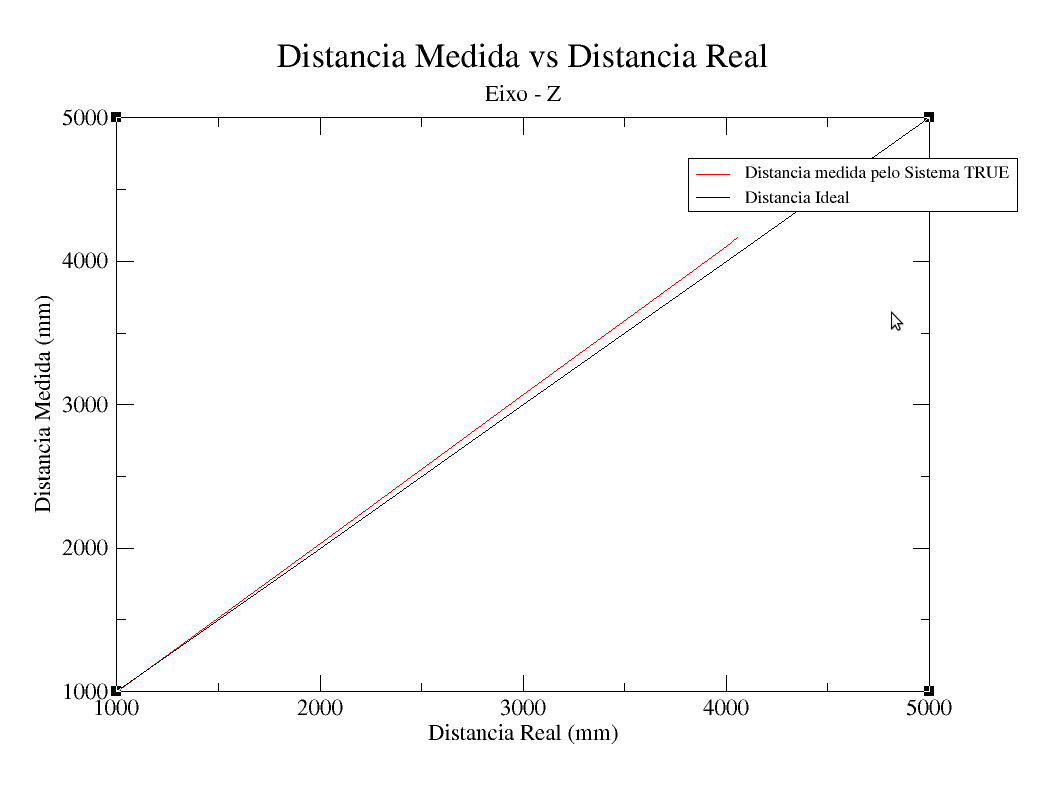
\includegraphics[scale=0.4]{figuras/5.Testes/grafico-eixo-z.png}
		\end{center}
		\caption{Gráfico comparativo entre os valores obtidos pelo Sistema TRUE e os
		valores reais para o eixo $\displaystyle z$.}
		\label{fig:grafico-z}
	\end{figure}

\subsection{Teste de localização para o eixo $\displaystyle x$}

	Os valores obtidos no eixo $\displaystyle x$ mostram o quanto o usuário
	rastreado está a direita ou a esquerda em relação ao \textit{Kinect}. Portanto,
	para testar a precisão do Sistema TRUE foi realizado o seguinte teste: um objeto
	(uma caixa de papelão) foi colocada a uma distância fixa de 3000 milímetros do
	sensor e colocada em diferentes posições ao longo do eixo $\displaystyle x$ (0,
	$\displaystyle \pm330mm$, $\displaystyle \pm660mm$, $\displaystyle \pm990mm$),
	como mostrado na Figura~\ref{fig:eixox-imgs}. Para cada posição, foram
	coletados os dados informados pelo sistema. A Tabela~\ref{tab:valores-x}
	apresenta o comparativo entre as distâncias reais medidas manualmente e a
	média das distâncias aferidas pelo sistema. Essa média aritmética é calculada
	a partir das amostras coletadas em um determinado período de tempo sendo
	algumas dessas escolhidas aleatoriamente para fazer parte da operação.

	% \begin{figure}[htb]
	% 	\begin{center}
	% 		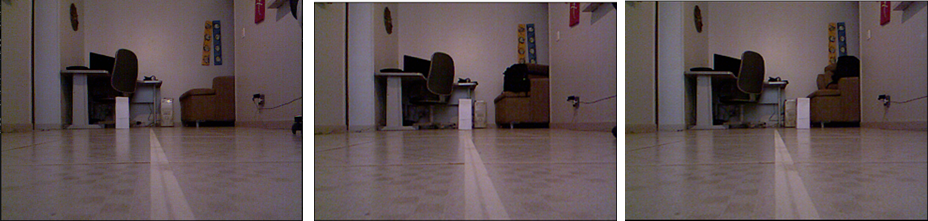
\includegraphics[scale=0.45]{figuras/5.Testes/teste-eixox.png}
	% 	\end{center}
	% 	\caption{Fotos retiradas no teste realizado para aferir os valores obtidos no eixo $\displaystyle x$.}
	% 	\label{fig:teste-eixox}
	% \end{figure}

	\begin{figure}[htb]
		\begin{center}
			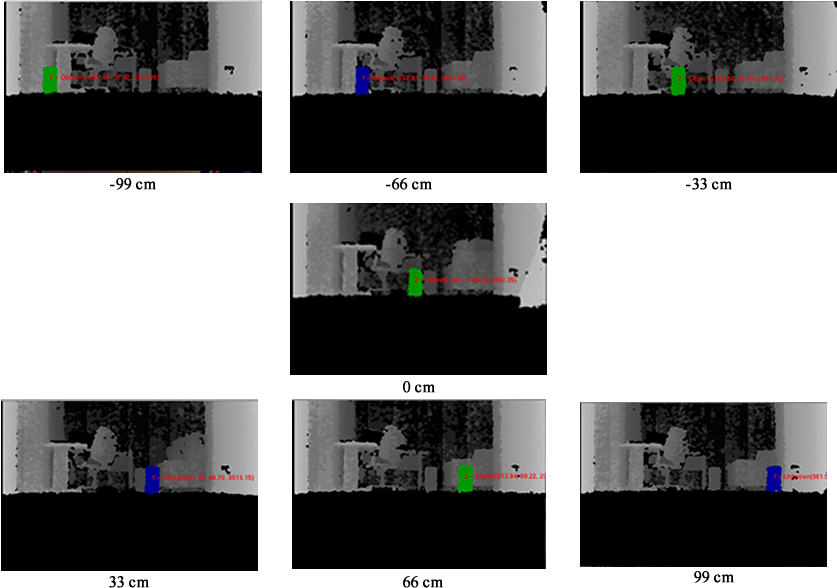
\includegraphics[width=0.95\textwidth]{figuras/5.Testes/eixox-imgs2.png}
		\end{center}
		\caption{Fotos obtidas pelo Sistema TRUE nos testes de localização para o eixo $\displaystyle x$.}
		\label{fig:eixox-imgs}
	\end{figure}

	\begin{table}[h]
		\begin{center}
			\caption{Comparativo entre as posições reais e os valores obtidos pelo Sistema TRUE.}
			\label{tab:valores-x}
			\begin{tabular}{|c|c|}
				\hline \bf Posição real do objeto & \bf Média dos valores obtidos}\\
							 \bf ao longo do eixo $\displaystyle x$ (mm) & pelo Sistema TRUE (mm)}\\
				\hline
				\hline 0    & -32,80 \\% -31,82   & -34,5    & -31,39   & -33,51 \\ 
				\hline 0    & -33,78 \\% -35,40   & -33,38   & -35,03   & -31,33  \\
				\hline 330  & 297,56 \\% 296,94   & 298,16   & 298,95   & 296,21 \\ 
				\hline -330 & -390,33 \\ % -387,42  & -391,42  & -392,54  & -389,96 \\ 
				\hline 660  & 615,10 \\%615,53   & 615,93   & 614,71   & 614,22 \\ 
				\hline -660 & -731,13 \\% -727,04  & -733,95  & -731,34  & -732,18 \\ 
				\hline 990  & 962,81 \\% 963,85   & 962,64   & 961,80   & 962,95 \\ 
				\hline -990 & -1069,29 \\% -1069,32 & -1068,00 & -1070,48 & -1069,35 \\
				\hline
			\end{tabular}
		\end{center}
	\end{table}
	
	Os valores da Tabela~\ref{tab:valores-x} também estão demonstrados graficamente
	na Figura~\ref{fig:grafico-eixox}. Como observado, existe uma diferença
	constante de poucos centímetros ao longo de toda a reta. É possível inferir
	então, que o Sistema TRUE consegue fazer estimativas das coordenadas no eixo
	$\displaystyle x$ com erro de poucos milímetros. Neste caso o menor e o maior
	erro obtidos foram de 27,19mm e 79,29mm respectivamente. Acredita-se que o
	erro apresentado não é significativo a ponto de comprometer o uso dos dados
	fornecidos.

	\begin{figure}[htb]
		\begin{center}
			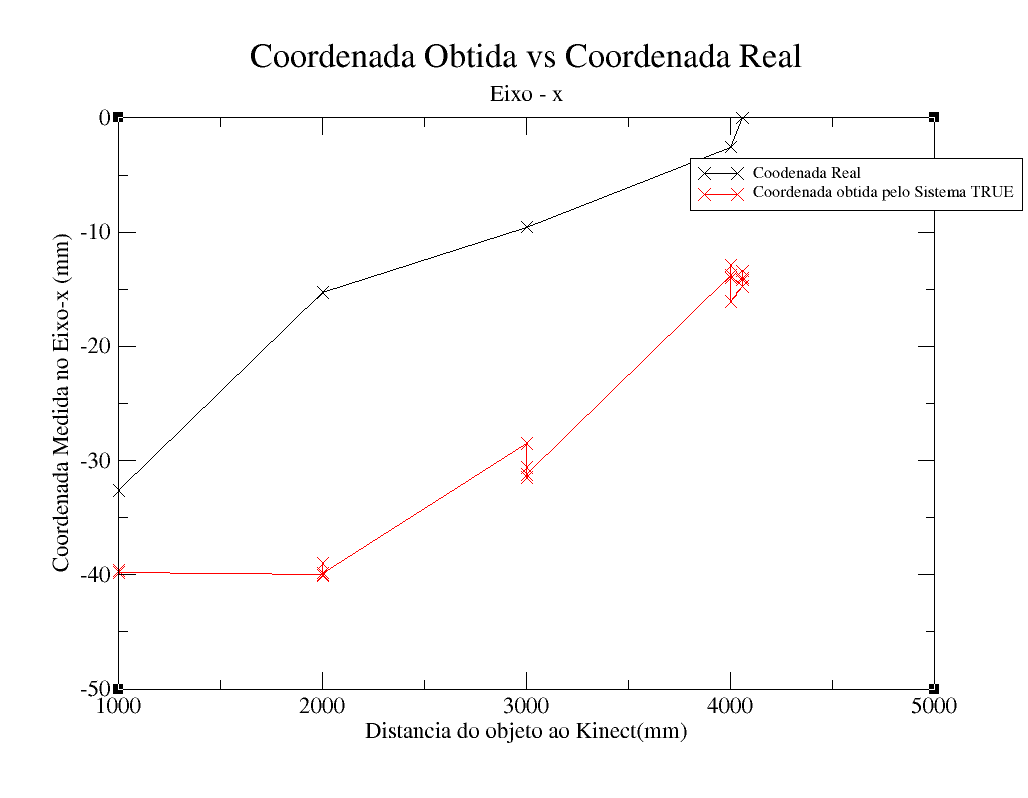
\includegraphics[scale=0.4]{figuras/5.Testes/grafico-eixo-x.png}
		\end{center}
		\caption{Gráfico comparativo entre os valores obtidos pelo Sistema TRUE e os valores reais para o eixo $\displaystyle x$.}
		\label{fig:grafico-eixox}
	\end{figure}
